% Compile: pdflatex paper_en.tex
\documentclass[10pt,twocolumn]{article}
\usepackage[a4paper,margin=18mm]{geometry}
\usepackage{graphicx}
\usepackage{amsmath}
\usepackage{amssymb}
\usepackage{booktabs}
\usepackage{enumitem}
\usepackage[hidelinks]{hyperref}

\setlength{\columnsep}{6mm}

\begin{document}

\twocolumn[{%
  \begin{center}
    {\LARGE\bfseries LoRA Fine-Tuning of a 12B-Parameter Image Generation Model for a Personally-Created Character}\\
    \vspace{0.6em}
    {\large FP8 Quantization and Block Swapping on a Single Consumer-Grade GPU, and Transfer to a Distilled Model}\\
    \vspace{1.2em}
    {\large Masato Suzuki (Masafy)}\\
    \vspace{0.4em}
    {June 25, 2026}
  \end{center}
  \vspace{1.0em}
  {\centering\textbf{Abstract}\par}
  \vspace{0.4em}
  \begingroup\small
  \noindent This report extends the author's prior work (LoRA fine-tuning of a character on Stable Diffusion 1.5) to \textbf{Krea~2}, a recent image-generation model roughly twelve times larger: a single-stream multimodal diffusion transformer (MMDiT) of the Qwen-Image family with about 12 billion parameters, trained with flow matching. Using the same subject (the author's personally-created red-panda character ``Masafee'') and the same hardware (a single NVIDIA GeForce RTX~3060 with 12\,GB of VRAM), we examine whether LoRA training of a 12-billion-parameter diffusion transformer is feasible on a single consumer-grade GPU. The key techniques are the joint use of (i) dynamic-scaled FP8 quantization of the 28 main blocks, (ii) block swapping of up to 26 blocks to the CPU, and (iii) PyTorch memory-fragmentation mitigation (\texttt{expandable\_segments}); together these keep the peak VRAM below 12\,GB. Training is performed on the pre-distillation RAW model, while inference uses the 8-step distilled Turbo model, forming a transfer configuration. From 13 reference images, 1{,}300 training steps ($\approx$8.4 hours) yielded the following: (a) identity-preserving character generation is achieved, and a LoRA trained on RAW transfers well to Turbo inference; (b) as the epoch count increases, the overall form is reinforced while \emph{high-frequency details}, such as the eye catchlights, are lost first, indicating overfitting; and (c) this degradation is recoverable at inference time by reducing the LoRA application strength and by text conditioning. The study demonstrates that, without paid cloud resources, additional training of a personal character on a state-of-the-art model at the 12-billion-parameter scale can be completed practically on a single consumer-grade GPU.

  \par\medskip
  \noindent\textbf{Keywords:}\ image generation, diffusion transformer, MMDiT, flow matching, low-rank adaptation, LoRA, FP8 quantization, block swapping, model distillation, consumer-grade GPU
  \endgroup
  \vspace{2.0em}
}]

\section{Introduction}
In prior work~\cite{suzuki2026sd15lora}, the author fine-tuned a personally-created original character ``Masafee'' (a red-panda character published as a messaging-app sticker set) onto the latent diffusion model Stable Diffusion~1.5 (SD~1.5; noise predictor of about 1 billion parameters) via Low-Rank Adaptation (LoRA), and showed that practical generation is possible on a single consumer-grade GPU with 12\,GB of VRAM.

Over the subsequent year, image-generation architectures shifted from U-Net-based latent diffusion to the \emph{diffusion transformer} (DiT)~\cite{peebles2023dit} and the \emph{multimodal diffusion transformer} (MMDiT)~\cite{esser2024sd3}, and the training objective moved from DDPM-style noise prediction to \emph{flow matching}~\cite{lipman2023flowmatching}. Krea~2, the target of this study, is a representative example: a single-stream MMDiT built on the Qwen-Image~\cite{qwenimage2025} family with about 12 billion parameters --- roughly twelve times the size of the SD~1.5 noise predictor used in the prior work.

A natural question arises: \emph{does the ``personal-character training on a single consumer-grade GPU'' framework still hold for a state-of-the-art model an order of magnitude larger?} Naively, a 12-billion-parameter model occupies about 24\,GB even in half precision (bf16), so even its weights do not fit on a 12\,GB GPU. Training is therefore fundamentally impossible without some memory-compression or offloading mechanism. The central contribution of this work is to overcome this constraint by jointly using FP8 quantization and block swapping, and to actually complete training. The specific research questions are:
\begin{itemize}[leftmargin=2.4em,topsep=2pt,itemsep=1pt]
  \item[\textbf{Q1.}] Can LoRA training of a 12-billion-parameter MMDiT --- whose weights alone require about 24\,GB in half precision --- be made feasible on a single GPU with 12\,GB of VRAM, and what are the necessary conditions?
  \item[\textbf{Q2.}] Does a LoRA trained on the pre-distillation RAW model transfer to inference on the few-step distilled Turbo model?
  \item[\textbf{Q3.}] How does increasing the epoch count change quality, and in particular do fine details (high-frequency) and overall form (low-frequency) behave the same way?
\end{itemize}
The contribution of this paper is to provide experimental answers to these questions together with a reproducible procedure.

\section{Related Work}
This work lies at the intersection of diffusion transformers, flow matching, low-rank adaptation, subject-driven generation, and memory-efficient training.

\textbf{Diffusion models and diffusion transformers.} The practical formulation of diffusion probabilistic models began with the DDPM of Ho et al.~\cite{ho2020ddpm}, and the latent diffusion model (LDM) of Rombach et al.~\cite{rombach2022ldm} improved the efficiency of high-resolution synthesis. Peebles and Xie~\cite{peebles2023dit} then replaced the U-Net with a transformer (DiT), and Esser et al.~\cite{esser2024sd3} introduced the MMDiT, which jointly processes image and text tokens, together with a rectified-flow objective. The single-stream MMDiT adopted by Krea~2 belongs to this lineage.

\textbf{Flow matching.} Lipman et al.~\cite{lipman2023flowmatching} proposed flow matching, which regresses a continuous normalizing flow from noise to data. Recent MMDiT-family models, including Krea~2, adopt this framework in place of DDPM-style noise prediction. The loss in this work (Eq.~\eqref{eq:fmloss}) is based on this formulation.

\textbf{Low-rank adaptation.} LoRA was proposed by Hu et al.~\cite{hu2022lora} as an efficient fine-tuning method for large language models, and was subsequently applied to transformers in general and to diffusion models. This work applies LoRA to the linear layers of an MMDiT.

\textbf{Subject-driven generation.} Binding a specific subject to a model from few reference images is called subject-driven generation, exemplified by the DreamBooth of Ruiz et al.~\cite{ruiz2023dreambooth}. The concept binding via the trigger token $\tau$ in this work follows this lineage.

\textbf{Memory-efficient training.} To handle a large model with limited VRAM, this work jointly uses low-precision numerics and per-layer offloading. FP8 was organized as a numerical format for deep learning by Micikevicius et al.~\cite{micikevicius2022fp8}. Block swapping (or offloading), which moves layers between CPU and GPU on demand, is a practical technique widely implemented in recent large generative-model trainers. The trainer used here, Musubi Tuner~\cite{musubi2026}, provides these in an integrated form.

\textbf{Model distillation.} Distilling multi-step diffusion/flow inference into few steps greatly reduces inference cost. Krea~2's Turbo is an 8-step distillation of RAW, and this work empirically examines the ``train on RAW, infer on Turbo'' transfer configuration.

\section{Background}
\subsection{Flow matching and the diffusion transformer}
Let an interpolation at time $t\in[0,1]$ between data $x_1\sim p_{\text{data}}$ and standard Gaussian noise $x_0\sim\mathcal{N}(0,\mathbf I)$ be given by the simplest straight path
\begin{equation}
x_t=(1-t)\,x_0 + t\,x_1 .
\label{eq:interp}
\end{equation}
The corresponding target velocity field is $v^\star=x_1-x_0$. A network $v_\theta$ regresses this field under condition $c$, and training minimizes the conditional flow-matching loss
\begin{equation}
\mathcal{L}(\theta)=\mathbb{E}_{x_0,\,x_1,\,t}\Big[\,\big\lVert v_\theta(x_t,t,c)-(x_1-x_0)\big\rVert_2^2\,\Big].
\label{eq:fmloss}
\end{equation}
At inference, one integrates the ordinary differential equation $\mathrm{d}x_t/\mathrm{d}t=v_\theta(x_t,t,c)$ from $t:0\to1$ along the learned velocity field. In Krea~2, $v_\theta$ is realized as a single-stream MMDiT in which image latent tokens and text condition tokens interact through shared self-attention layers. The condition $c$ is an intermediate-layer feature of the text encoder (Qwen3-VL-4B), and the image autoencoder is the Qwen-Image VAE.

\subsection{Resolution-dependent time shift}
In flow-based models, skewing the distribution of the training time $t$ according to resolution contributes to quality. We use a \emph{shift} given by the monotone map
\begin{equation}
t' = \frac{\sigma\, t}{1+(\sigma-1)\,t},
\label{eq:shift}
\end{equation}
where $\sigma$ is the shift coefficient; at $1024\times1024$, $\sigma=2.5$ matches the inference-time shift of Krea~2 (see below).

\subsection{Low-rank adaptation}
A linear-layer weight $W_0\in\mathbb{R}^{d_\text{out}\times d_\text{in}}$ is frozen, and only the low-rank difference $\Delta W=BA$ ($A\in\mathbb{R}^{r\times d_\text{in}},\,B\in\mathbb{R}^{d_\text{out}\times r}$, $r\ll\min(d_\text{in},d_\text{out})$) is trained. The forward pass is
\begin{equation}
h = W_0 x + \frac{\alpha}{r}\,B A x ,
\label{eq:lora}
\end{equation}
where $\alpha$ is a scaling coefficient. At inference, introducing an application strength $\lambda$ as $h=W_0x+\lambda\,\frac{\alpha}{r}BAx$ allows the LoRA effect to be tuned continuously after training. This work uses $\lambda$ as a means of quality control (Section~\ref{sec:results}).

\subsection{Memory efficiency via FP8 quantization and block swapping}
\label{sec:mem}
A 12-billion-parameter model occupies about 24\,GB in bf16 and does not fit on a 12\,GB GPU. This work overcomes this by jointly using the following three.
\textbf{(i) FP8 scaled quantization.} The weights of the 28 main blocks of the MMDiT are quantized at load time to dynamic-scaled FP8 (E4M3), roughly halving the weight memory. Auxiliary parts including normalization layers are kept in bf16.
\textbf{(ii) Block swapping.} Up to 26 of the main blocks ($=28-2$) are kept resident in CPU main memory and transferred to the GPU only immediately before computation, further reducing GPU-resident weights.
\textbf{(iii) Fragmentation mitigation.} PyTorch's caching allocator is switched to \texttt{expandable\_segments} mode so that reserved-but-unallocated fragments can be reused.
During training, the text-encoder and VAE outputs are precomputed and offloaded to disk, so that only the MMDiT occupies the GPU in the training step itself.

\section{Problem Setting}
From the full set of 16 ``Masafee'' stickers created by the author, 13 are selected by quality criteria as the training set $\mathcal{D}=\{(x^{(i)},y^{(i)})\}_{i=1}^{13}$. Each $y^{(i)}$ is a tag-style caption with the trigger token $\tau=\texttt{masafee}$ placed first. The goal is to learn LoRA parameters $\phi=\{A_\ell,B_\ell\}_\ell$ from $\mathcal{D}$ and, at inference, generate identity-preserving images for text $y$ specifying unrecorded poses and scenes. For a fair comparison with the prior work, the subject, GPU, trigger token, and data selection (13 images) are kept identical to the prior work, restricting the difference to the architecture (SD~1.5 $\to$ Krea~2) and the training stack.

\section{Method}
\subsection{Model and data preparation}
The diffusion model is Krea~2 RAW (a single \texttt{safetensors}, about 24\,GB). The text encoder is Qwen3-VL-4B (bf16) and the autoencoder is the Qwen-Image VAE. Prior to training, we perform (1) precaching of image latents via the VAE and (2) precaching of text-encoder outputs, to avoid keeping the encoder and VAE resident during the training step. Training images are bucketed to $1024\times1024$ (the originals are $1000\times1000$).

\subsection{Training configuration}
LoRA is inserted into the linear layers of the MMDiT with rank $r=32$ and $\alpha=32$. Optimization uses AdamW, learning rate $1\times10^{-4}$, batch size 1, and gradient checkpointing enabled. Time sampling uses the shift (Eq.~\eqref{eq:shift}, $\sigma=2.5$), and the loss is Eq.~\eqref{eq:fmloss}. The total number of steps is $13\times10=130$ steps/epoch $\times$ 10 epochs $=1{,}300$ steps. To meet the VRAM constraint, all of (i)--(iii) in Section~\ref{sec:mem} are applied, with the block-swap count set to its maximum of 26. Intermediate checkpoints are saved every 2 epochs.

\subsection{Inference configuration and transfer}
Inference uses the 8-step distilled Turbo (GGUF~Q5\_K\_M quantization for memory savings). The LoRA trained on RAW is applied to the Turbo MMDiT, and generation uses sampler \texttt{er\_sde}, scheduler \texttt{simple}, 8 steps, and guidance scale $s=1.0$ (Turbo is CFG-free). This realizes a configuration in which training is performed on the high-precision RAW while inference is performed on the fast, memory-efficient Turbo.

\section{Experiments}
Training and inference were completed entirely on a single consumer-grade GPU (NVIDIA GeForce RTX~3060, 12\,GB VRAM, driver 595.71.05) installed in a home Linux PC (30\,GB main memory, PyTorch 2.6.0+cu124). No paid cloud computing resources were used. During training, GPU power, temperature, VRAM occupancy, and throughput were recorded. Evaluation is along three axes: (E1) feasibility of training and resource behavior, (E2) identity acquisition and RAW$\to$Turbo transfer, and (E3) ablation over epochs and quality control by inference-time intervention. In generation comparisons, the same prompt and same random seed are used to make epoch differences explicit.

\section{Results}
\label{sec:results}
\subsection{E1: Feasibility of training and resource behavior}
With the joint use of the three techniques in Section~\ref{sec:mem}, LoRA training of the 12-billion-parameter MMDiT \emph{was feasible} on a single GPU with 12\,GB of VRAM. The peak VRAM occupancy was about 11.9\,GB (about 97\% of capacity), fitting within 12\,GB with a small margin. Notably, without the fragmentation mitigation \texttt{expandable\_segments}, training stopped at step 2 upon failing to allocate an additional $\sim$136\,MiB (while about 1.4\,GiB was stuck as reserved-but-unallocated fragments). That is, at this scale, the fragmentation mitigation --- in addition to FP8 quantization and block swapping --- was an \emph{effective necessary condition}.

The training throughput was about 23.2\,s/step, and the total time for 1{,}300 steps was 8 hours 23 minutes. Figure~\ref{fig:loss} shows the training-loss trajectory. The loss rose early, then decreased monotonically and plateaued at about 0.027 toward the end. The GPU ran at nearly 100\% utilization throughout, with temperature in the safe range of 69--75\,$^\circ$C and power draw at 135\,W (about 80\% of the 170\,W limit). These show that a consumer-grade GPU can sustain training at this scale with thermal and power headroom.

\begin{figure}[t]\centering
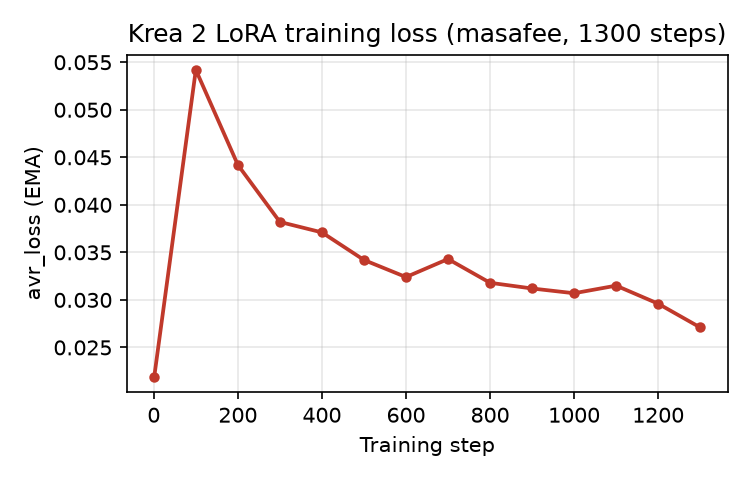
\includegraphics[width=0.96\columnwidth]{figures/fig_loss.png}
\caption{Training loss (exponential moving average). It rises early, then decreases monotonically and plateaus at about 0.027. Total 1{,}300 steps, about 8.4 hours.}
\label{fig:loss}
\end{figure}

\subsection{E2: Identity acquisition and RAW$\to$Turbo transfer}
Figure~\ref{fig:identity} compares no-LoRA (base Turbo) and LoRA-applied generation under the same prompt and seed. The base only produces a generic red panda, whereas applying the LoRA consistently reproduces Masafee-specific designs such as goggles, a crown-pattern outfit, and a striped tail. Since the LoRA trained on RAW works directly in the 8-step Turbo inference, we conclude that the \emph{RAW$\to$Turbo transfer holds well}. This shows that the division of labor --- training on a high-precision model and inferring on a distilled model --- is practically effective.

\begin{figure}[t]\centering
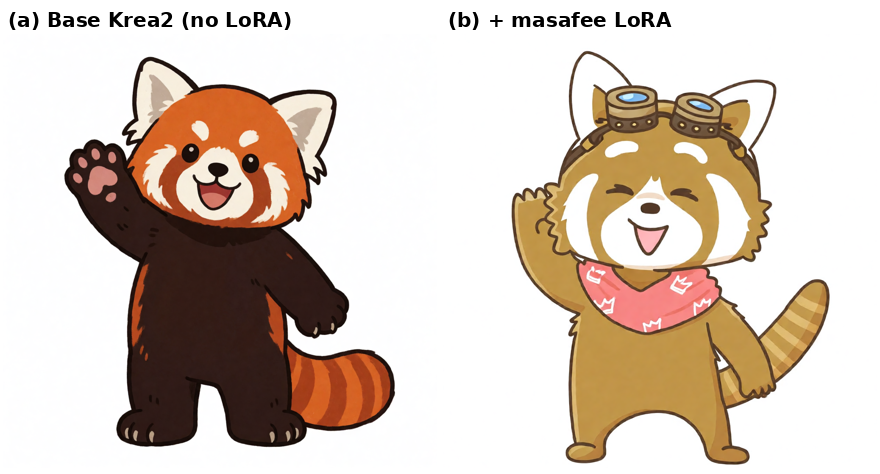
\includegraphics[width=0.96\columnwidth]{figures/fig_identity.png}
\caption{Comparison under the same prompt and seed. Left: no LoRA (base). Right: with LoRA. The latter reproduces signature designs such as goggles, a crown-pattern outfit, and a striped tail.}
\label{fig:identity}
\end{figure}

\subsection{E3: Epoch ablation and degradation of high-frequency details}
Figure~\ref{fig:epoch} arranges generations of 6 poses $\times$ 3 epochs (6/8/10) under the same seed. Identity is preserved across all epochs and generalizes to arbitrary poses. However, a systematic difference is observed across epochs. Epoch 10 has the strongest and most stable overall form (body shape, outfit, color), but shows signs of overfitting: (a) the background drifts toward the warm-color gradient seen in the training data, and (b) the eye catchlights (white highlight dots) are lost. By contrast, epochs 6 and 8 follow the prompt instruction (plain background) more readily and preserve the eye catchlights.

Notably, overfitting first appears in \emph{high-frequency details} (the few-pixel catchlights), while the low-frequency overall form is instead reinforced. The catchlight is a small feature whose appearance is unstable across the 13 training images; it can be interpreted as being averaged out and overwritten as the LoRA effect strengthens. Figure~\ref{fig:eye} shows this phenomenon at a magnified scale.

\begin{figure*}[t]\centering
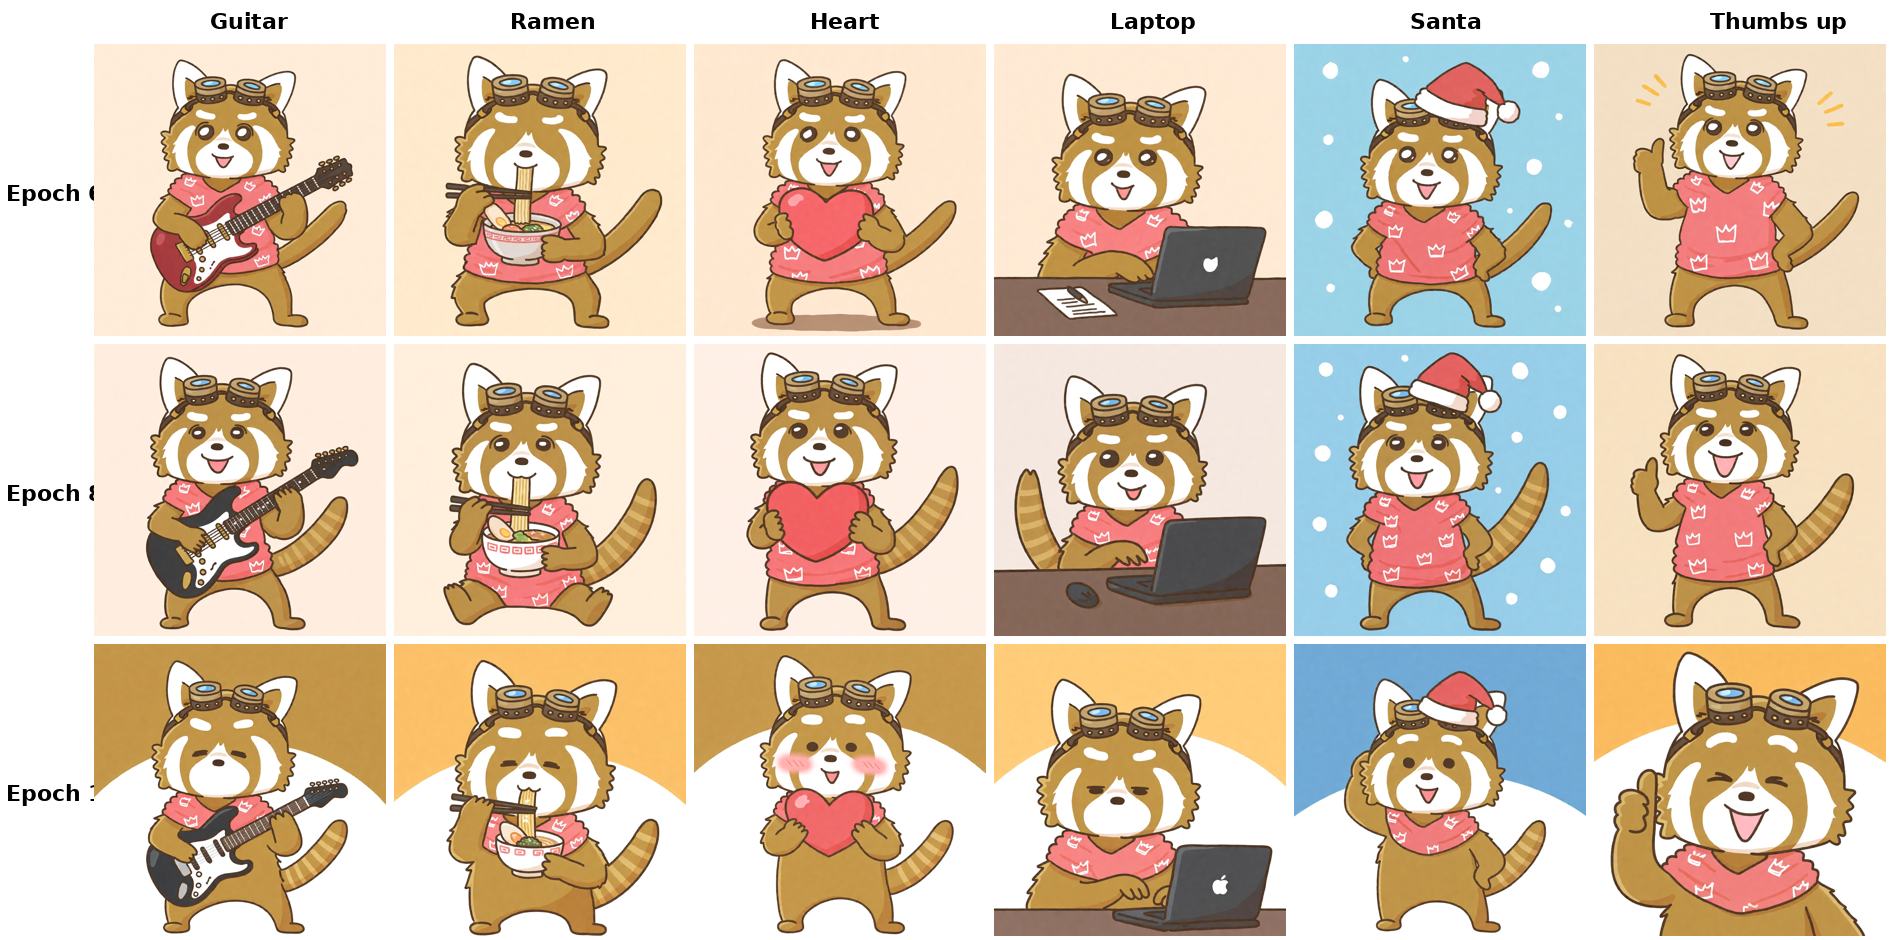
\includegraphics[width=0.92\textwidth]{figures/fig_epoch.png}
\caption{Epoch ablation (rows: epochs 6/8/10; columns: 6 poses; same seed). Epoch 10 has the strongest overall form but shows overfitting: backgrounds drift toward warm colors and the eye catchlights are lost.}
\label{fig:epoch}
\end{figure*}

\subsection{Quality control by inference-time intervention}
We examined whether the form and the details of epoch 10 can be reconciled by inference-time intervention alone. Figure~\ref{fig:eye} compares (A) epoch 10 with application strength $\lambda=1.0$, (B) epoch 10 with $\lambda=0.8$, (C) epoch 10 with $\lambda=1.0$ plus a prompt that explicitly specifies eye highlights, and (D) epoch 8 with $\lambda=1.0$ as a reference. Reducing $\lambda$ (B) loosens the overfitting effect and partially recovers the details, while prompt conditioning (C) brings back the catchlights while preserving the epoch-10 form. Combining the two ($\lambda=0.8$ plus prompt) gave the best compromise between overall form and high-frequency detail. This shows that, without retraining, the side effects of overfitting can be controlled practically using two inference-time degrees of freedom: the application strength ($\lambda$ in Eq.~\eqref{eq:lora}) and the text condition.

\begin{figure}[t]\centering
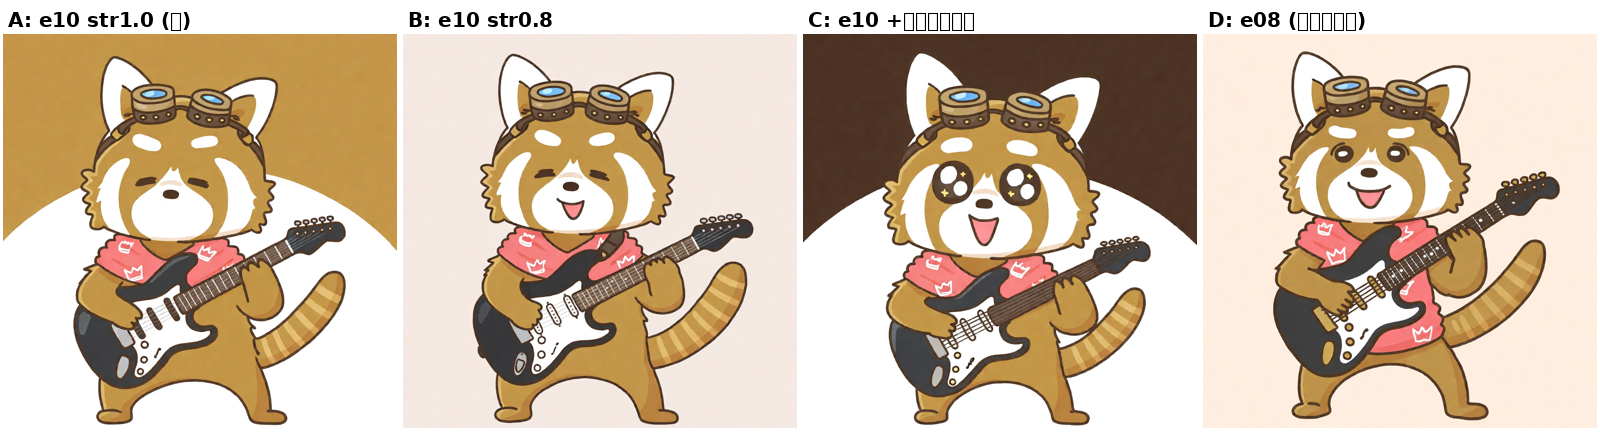
\includegraphics[width=0.96\columnwidth]{figures/fig_eye.png}
\caption{Recovery of eye catchlights. (A) e10, $\lambda{=}1.0$; (B) e10, $\lambda{=}0.8$; (C) e10, $\lambda{=}1.0$ plus eye-highlight prompt; (D) e8 (reference). Reducing $\lambda$ and prompt conditioning recover high-frequency detail.}
\label{fig:eye}
\end{figure}

\section{Discussion}
\textbf{Robustness of the framework to scale.} The prior work~\cite{suzuki2026sd15lora} demonstrated personal-character training of a $\sim$1-billion-parameter U-Net on a consumer-grade GPU. This work extends it to a $\sim$12-billion-parameter MMDiT --- about 12 times larger --- and shows that the framework still holds on the same GPU. The differences lie in the scale of the training target and the numerical/memory strategy; the subject, data size, and GPU are shared. Thus the claim ``additional training of a personally-owned character can be completed on a single consumer-grade GPU'' was robust across generations.

\textbf{Frequency asymmetry of overfitting.} The phenomenon observed in E3 --- high-frequency details degrade before the low-frequency form --- provides a guideline for epoch selection in few-shot character LoRA. The final epoch is not necessarily the best; if detail preservation is prioritized, an earlier epoch or a reduced inference-time application strength is effective. Crucially, this degradation is not destructive and can be reversibly compensated using two inference-time degrees of freedom ($\lambda$ and the text condition).

\textbf{Division of labor between training and inference.} Training on RAW and inferring on Turbo reconciles the numerical stability of training (high-precision RAW) with inference efficiency (8-step, memory-efficient Turbo). When a distilled model is hard to use as a training target, assigning the pre-distillation model to training, as in this configuration, can serve as a general guideline.

\section{Limitations and Future Work}
This work has the following limitations. First, throughput is about 23.2\,s/step, much larger than for SD~1.5 training, dominated by the CPU--GPU transfers of block swapping. Second, block swapping pressures main memory and required temporarily pausing other GPU/memory-resident services during training. Third, the evaluation is mainly qualitative; quantitative identity metrics (e.g., embedding similarity) and human evaluation are future work. Fourth, checkpoints were saved only every 2 epochs, so the exact boundary at which overfitting emerges was not pinpointed. Fifth, inference also uses quantization (GGUF~Q5\_K\_M), and the effect of quantization on transfer quality was not isolated.

\section{Conclusion}
This work demonstrated that LoRA fine-tuning of a personal character on Krea~2 --- a state-of-the-art image-generation model with about 12 billion parameters --- is feasible on a single consumer-grade GPU (RTX~3060, 12\,GB VRAM). The joint use of FP8 quantization, block swapping, and memory-fragmentation mitigation was a necessary condition for training at this scale, and a LoRA trained on the pre-distillation RAW transferred well to inference on the distilled Turbo. Furthermore, we observed a frequency asymmetry of overfitting in which increasing the epoch count degrades high-frequency details first, and showed that this is reversibly compensable via inference-time application strength and text conditioning. The conclusion of the prior work --- that additional training of a personal character can be completed on a single consumer-grade GPU without paid cloud resources --- continues to hold for a latest-generation model an order of magnitude larger.

\section*{Appendix A: Key Hyperparameters}
Diffusion model: Krea~2 RAW (training) / Turbo GGUF~Q5\_K\_M (inference). Text encoder: Qwen3-VL-4B (bf16). VAE: Qwen-Image VAE. LoRA: rank $r=32$, $\alpha=32$, applied to MMDiT linear layers. Optimization: AdamW, learning rate $1\times10^{-4}$, batch size 1, gradient checkpointing enabled. Time sampling: shift, $\sigma=2.5$. Total steps: 1{,}300 (10 epochs). Memory efficiency: FP8 scaled quantization + block swap 26 + \texttt{expandable\_segments}. Resolution: $1024\times1024$. Inference: \texttt{er\_sde} / \texttt{simple} / 8 steps / $s=1.0$. Adopted setting: epoch 10, application strength $\lambda=0.8$, combined with a prompt specifying eye highlights.

\section*{Appendix B: Reproduction Environment}
GPU: NVIDIA GeForce RTX~3060 (12\,GB VRAM, driver 595.71.05). Main memory: 30\,GB. PyTorch: 2.6.0+cu124. Training stack: Musubi Tuner~\cite{musubi2026} (commit \texttt{30c658c}). Training time: 8 hours 23 minutes (about 23.2\,s/step). Final loss: 0.0269.

\begin{thebibliography}{9}
\bibitem{suzuki2026sd15lora} M.~Suzuki. LoRA Fine-Tuning of a Personally-Created Character for Image Generation: An Empirical Study under Few-Shot Conditions on a Consumer-Grade GPU. Technical report, 2026.
\bibitem{ho2020ddpm} J.~Ho, A.~Jain, and P.~Abbeel. Denoising Diffusion Probabilistic Models. \textit{Advances in Neural Information Processing Systems (NeurIPS)}, 2020.
\bibitem{rombach2022ldm} R.~Rombach, A.~Blattmann, D.~Lorenz, P.~Esser, and B.~Ommer. High-Resolution Image Synthesis with Latent Diffusion Models. \textit{IEEE/CVF Conference on Computer Vision and Pattern Recognition (CVPR)}, 2022.
\bibitem{peebles2023dit} W.~Peebles and S.~Xie. Scalable Diffusion Models with Transformers. \textit{IEEE/CVF International Conference on Computer Vision (ICCV)}, 2023.
\bibitem{esser2024sd3} P.~Esser, S.~Kulal, A.~Blattmann, et al. Scaling Rectified Flow Transformers for High-Resolution Image Synthesis. \textit{International Conference on Machine Learning (ICML)}, 2024.
\bibitem{lipman2023flowmatching} Y.~Lipman, R.~T.~Q. Chen, H.~Ben-Hamu, M.~Nickel, and M.~Le. Flow Matching for Generative Modeling. \textit{International Conference on Learning Representations (ICLR)}, 2023.
\bibitem{hu2022lora} E.~J.~Hu, Y.~Shen, P.~Wallis, Z.~Allen-Zhu, Y.~Li, S.~Wang, L.~Wang, and W.~Chen. LoRA: Low-Rank Adaptation of Large Language Models. \textit{International Conference on Learning Representations (ICLR)}, 2022.
\bibitem{ruiz2023dreambooth} N.~Ruiz, Y.~Li, V.~Jampani, Y.~Pritch, M.~Rubinstein, and K.~Aberman. DreamBooth: Fine Tuning Text-to-Image Diffusion Models for Subject-Driven Generation. \textit{IEEE/CVF Conference on Computer Vision and Pattern Recognition (CVPR)}, 2023.
\bibitem{qwenimage2025} Qwen Team. Qwen-Image Technical Report. 2025.
\bibitem{micikevicius2022fp8} P.~Micikevicius, D.~Stosic, N.~Burgess, et al. FP8 Formats for Deep Learning. arXiv:2209.05433, 2022.
\bibitem{musubi2026} kohya-ss. Musubi Tuner. \url{https://github.com/kohya-ss/musubi-tuner}, 2026.
\end{thebibliography}

\end{document}
